\section{Discussion}

\subsection{Humans as Sensors}

`Humans as sensors` defines a new measurement model for crowdsensing. In the model, measurements are
not only taken by smartphone, but also come from the personal observations of participants. 
As a complement of automatically acquiring the localization data from smartphones, ThunderLoc provides the interface for participants to manually upload personal observations.
The users of smartphones can manually input the personal localization data in the ThunderLoc app, 
including the binary left/right data, the position and direction when they hear the thunder.

However, how to motivate enough participants for ThunderLoc is a problem in reality. 
%The incentive mechanisms for smartphone collaboration are out of range of the paper. 
Here a possible solution is given as follows. ThunderLoc app can be integrated into a weather forecast app. When the thundershower is coming, 
the weather forecast app pushes a notice to inquire whether the user to join the ThunderLoc project. 
If the user agrees to participate in, ThunderLoc app will be downloaded and run. Once the cloud platform finishes the localization operation,
the position of thunder will be push to the user. 
The well-informed discussions about the incentive mechanisms for smartphone collaboration are detailed in Ref.~\cite{duan2012incentive}.


\subsection{The Impact of Background Noises}
Above, we put forward basic ThunderLoc and robust ThunderLoc to implement thunder localization by using dual-microphone smartphones.
The binary left/right measurement data of each smartphone is from the sign of TDOA between two audio signals recorded with dual-microphone. 
However, in the practical localization system, bit-flip problem may occur because of the effect of background noises in the phase of computing binary left/right data for each smartphone,
then lead to localization error.

%In the presence of background noise, 
%some of the peaks in related to reflective paths might have a magnitude that turns out to be comparable to or larger than that of the direct path. 
%For this reason, we use the reliability index that computes the ratio between the energy in a window containing the highest peak and the energy of the remaining samples in GCC-PHAT:

%\begin{equation}
%F(i) = \frac{{\sum\nolimits_{\tau  \in W} {R_{m_i^1,m_i^2}^2}(\tau ) }}{{\sum\nolimits_{\tau  \notin W} {R_{m_i^1,m_i^2}^2} (\tau )}}
%\end{equation}
%where $W$ is an interval around the highest peak in the GCC-PHAT algorithm.

\iffalse
  \begin{figure}[ht]
            \setlength{\abovecaptionskip}{0pt}
            \centering
            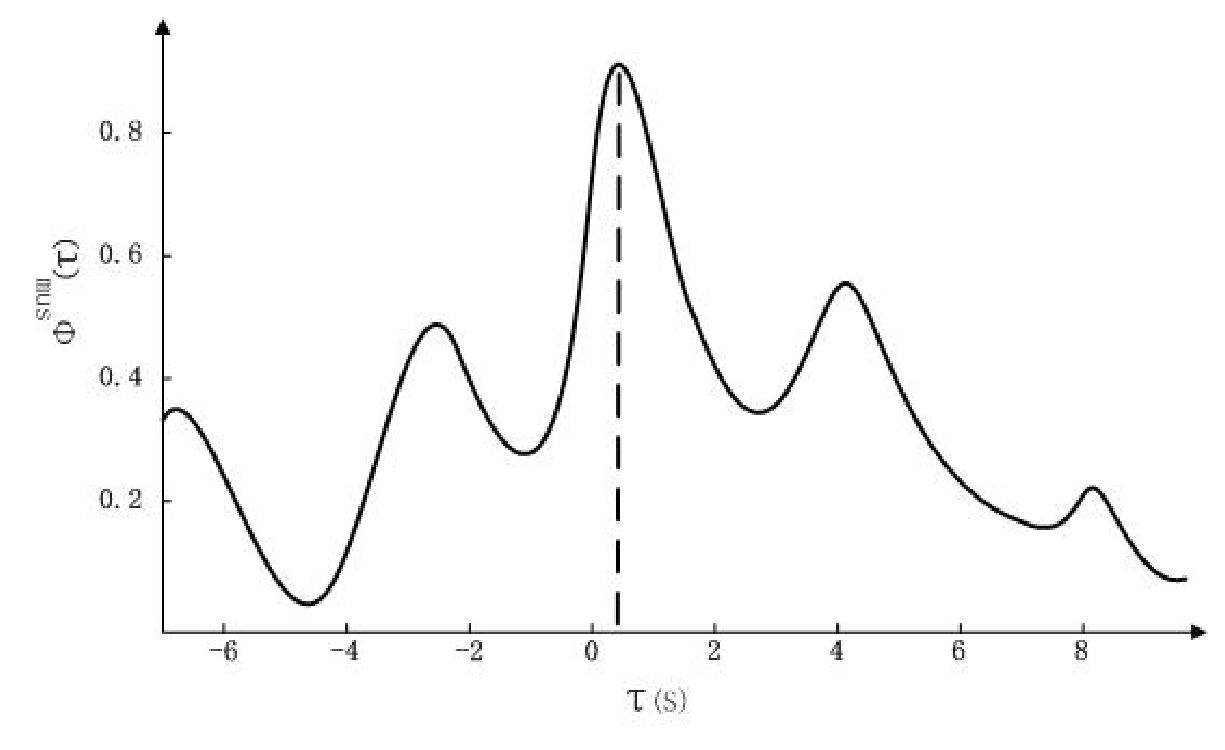
\includegraphics[scale=1.4,height=4.0cm]{image/tde.eps}
            \caption{weight calculation.}
            \label{weighting}
            \vspace{-1mm}
  \end{figure}
  \fi
 


Considering the impact of background noises, we use the SNR of each smartphone node as the reliability metric, then compute Hamming distance with the reliability informatio
%In the presence of background noise, 
The lower SNR is near the smartphone, the binary left/right measurement data of the smartphone is more unreliable.   
Moreover, when the estimated TDOA is far from zero, the result of 1-bit quantization is more reliable. 
The framework of the improved localization is the same as proposed robust localization described in Algorithm \textbf{1}, 
the only difference between them is that Hamming distance is substituted by weighting Hamming distance with the reliability metric.
% \begin{equation}
% WHD = \sum\limits_{i = 1}^N {F(i) \left( T(i) \oplus D_j(i)\right)}
% \end{equation}

 \vspace{-2mm}   
\subsection{System Scalability and Multiple Thunder Localization}

ThunderLoc system can achieve higher localization performance as the number of smartphones increases,
such extensibility is a unique advantage compared with dedicated microphone array hardware.

Our system is evaluated in the small campus area, but it can extend to large area. 
In Fig.11, the signal from thunder in large-scale system only can cover limited area which means when we measure the binary sequence, 
 just a small portion of microphones close to the thunder are effective. 
So the binary sequence of thunder is shorter than $N$ (there exist $N$ dual-microphone smartphones). 
We can use a range R to put the large-scale system down to a smaller area which is large enough to cover the coverage of the thunder's signal. 
And the small area can be handled as our algorithm proposed by preceding part of the paper. 
By this way, the length of the binary sequence is shorter and matching is more efficient.


Localizing multiple, simultaneously active acoustic sources is a more difficult task. 
In order to avoid conflict of several acoustic sources, 
multiple source localization must be able to uniquely identify the signature of each thunder. 
%which is beyond the capability of this paper, and we will not do too much discussion about it in this paper. 
For example, if the several thunders are set as shown in Fig. \ref{multiple_source_localization},
we can calculate the positions of the two thunders because the thunder I is far enough from thunder II. 
The smartphones close to effective area I could handle thunder I, and another smartphones close to effective area II could handle thunder II. 
  \vspace{-8mm}
  \begin{figure}[ht]
            \setlength{\abovecaptionskip}{0pt}
            \centering
            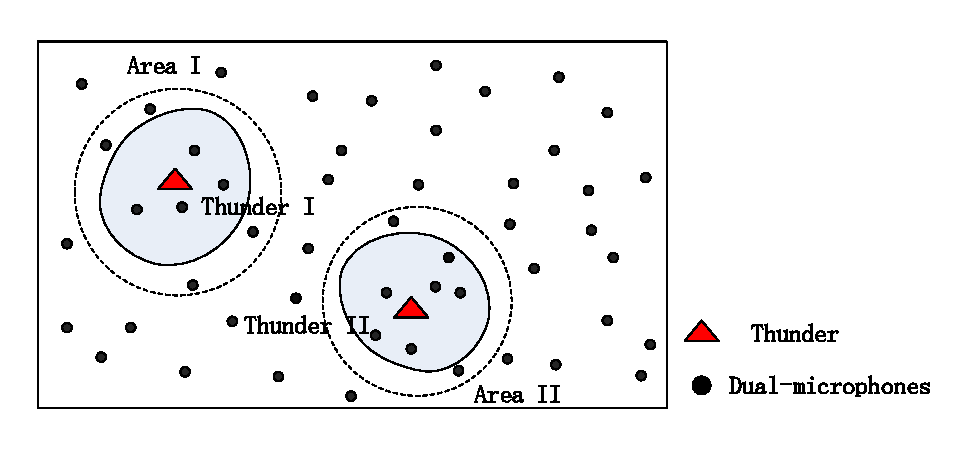
\includegraphics[scale=1.2,height=3.2cm]{fig/msl.pdf}
             \vspace{1mm}
			\caption{\label{Fig9:} System scalability for large-scale systems.}
            \label{multiple_source_localization}
            \vspace{-1mm}
  \end{figure}

 \vspace{-8mm}
 
\subsection{Time Synchronization and Energy Efficiency}
In our system, we calculate the sign of TDOA by utilizing two synchronized audio signals from dual-microphone of each smartphone. 
%Time synchronization among smartphones is not in high demand to locate the thunder, which is already supported in the recent 4G cellular network.
High-accuracy of time synchronization among smartphones is not required.

Energy efficiency is another issue in smartphone networks.
We can activate the ThunderLoc app in the smartphone according to the thundershower alert from the weather forecast app.
Only if it is raining with thunder, ThunderLoc app will be awake.






